\section{Experiments and Discussion}
\label{sec:Experiment}

In this chapter, we conduct experiments to evaluate our methods proposed
in \ref{sec:ClassificationMethod1} and \ref{sec:ClassificationMethod2},
and present the results obtained from them.  In addition, we discuss our
methods based on the results.

\subsection{Data Set}
\label{subsec:Data Set}

We collected the data set from the real Twitter data by using Twitter
API.

We first randomly selected 1,000 Twitter users whose timezone is Japan.
At this time, we omitted users who are followed from nobody and who post
no tweet in order to select only active users.  Then, we divided them in
two sets equally, i.e., each of which include 500 users.

Second, we had 6 experienced Twitter users as participants, all of whom
are male graduate students in engineering, from 23 to 25 years old.  We
assigned each set to 3 participants, and we asked each participant to
determine one of the following categories each user in the assigned set
is supposed to be in:

\begin{description}
\item[(i)] the user publishes information to the public widely,
\item[(ii)] the user publishes information specified for certain topics,
\item[(iii)] the user publishes information to the users specified
           extensionally, and
\item[(iv)] the user publishes information (ii) specified for certain
           topics (iii) to the users specified extensionally.
\end{description}

\noindent{These categories correspond to the category (b), (1), (2), (3)
in Figure~\ref{fig:Flow} respectively.}

Then, we selected users whose category at least 2 out of 3 participants
coincide with, and as a result, we were able to collect 93, 320, 375,
and 30 users in the category (i), (ii), (iii), and (iv).  We randomly
selected 90 users from the category (i), and 30 users from (ii), (iii),
and (iv) respectively.  We collected these 180 users in total, and we
used them as the data set.  Table~\ref{table:breakdown} shows the
breakdown of the data set: average and standard deviation of numbers of
followers,  followees, and tweets in each category.

\newcolumntype{I}{!{\vrule width 1.5pt}}
\newcommand{\bhline}[1]{\noalign{\hrule height #1}}
\begin{table}[t]
\caption{Average and standard deviation of numbers of followers,
 followees, and tweets in each category \label{table:breakdown}}
\begin{center}
\begin{tabular}{c|cIc|c|c|c}
\multicolumn{2}{cI}{} & \makebox[4em]{i} & \makebox[4em]{ii} &
 \makebox[4em]{iii} & \makebox[4em]{iv} \\ \bhline{1.5pt}
 \multirow{2}{*}{follower} & average & 475,679 & 58,142 & 573 & 82,942  \\
 & standard deviation & 535,894 & 171,784 & 1,389 & 262,161 \\ \hline
 \multirow{2}{*}{followee} & average & 11,274 & 3,353& 598 & 1,568 \\
 & standard deviation & 37,906 & 7,218 & 1,545 & 3,594 \\ \hline
 \multirow{2}{*}{tweet} & average & 9,763 & 9,992 & 8,829 & 5,677 \\
 & standard deviation & 14,607 & 23,572 & 29,505 & 6,600 \\
\end{tabular}
\end{center}
\end{table}

Then, for each user, we collected at most 1,000 followers of the user,
and in regard to the followers who follow at most 1,000 users, we also
collected their followees.  We used them in order to evaluate our
methods.

\subsection{Experimental Settings and Libraries}
\label{subsec:Settings}

First, we conducted the experiments evaluating the method of classifying
Twitter users based on the target specificity of their information
publishing mentioned in \ref{sec:ClassificationMethod1}.  We used 90
users classified into the category (i) as target users, and 90 users
classified into the category (ii), (iii), and (iv) as non target users.
We first computed $\mathit{SpecificityScore}_{{\mathit{term}}}(u)$ and
$\mathit{SpecificityScore}_{{\mathit{followee}}}(u)$ for each user $u$,
and computed $\mathit{TargetSpecificity}(u)$ based on the above scores.
Then, we determined a threshold $\delta$ which can classifies target
users and non target users accurately the most, and evaluated the
classification results with $\delta$.  When computing
$\mathit{TargetSpecificity}(u)$, we used two models: the probabilistic
model and the subtracting model mentioned in \ref{subsec:Scoring}, and
compared them.

Second, we conducted the experiments evaluating the method of determing
why the target specificity of the user is high in regard to the target
user mentioned in \ref{sec:ClassificationMethod2}.  We extracted users
from the category (ii), (iii), and (iv) by 30 users, and used 90 users
in total.  We first extracted features mentioned in
\ref{sec:ClassificationMethod2} from the user, which are normalized to a
value between $0$ and $1$.  Then, based on these features, we
constructed two types of classifiers: a single 3-class classifier and
two binary classifiers, which classify users into three categories:
(ii), (iii), and (iv), and evaluated the classification results using
3-fold cross validation.  We used two learning algorithms: SVM and the
decision tree as classifiers, and compared them.  For SVM, we used
LIBSVM\footnote{\url{http://www.csie.ntu.edu.tw/~cjlin/libsvm/}}, which
is a popular SVM library, with the Gaussian kernel, which using
one-against-one method for multiclass classification.  For the decision
tree, we used scikit-learn
\footnote{\url{http://scikit-learn.org/stable/modules/tree.html}}.

We used twpro search API\footnote{\url{http://twpro.jp/doc/api/search}}
in order to get a number of users who have a certain term in their
profiles.  We also used
MeCab\footnote{\url{http://mecab.sourceforge.net/}} for morphological
analysis of Japanese sentences in profiles, local information, and
tweets of users.  Furthermore, we used
gensim\footnote{\url{http://radimrehurek.com/gensim/}} for using Latent
Dirichlet Allocation (LDA).

\subsection{Results and Evaluation of Classifying Users Based on Target
  Specificity}
\label{subsec:Results of Method1}

In this subchapter, we show the results of the experiments classifiying
users based on target specificity of their information publishing.

\begin{table}[t]
\caption{Precision of the classification of target users and non target
 users using a couple of attributes measuring consistency separately
 \label{table:Classify Target Users}}
\begin{center}
\begin{tabular}{cIccc|c}
 & \multicolumn{3}{c|}{Probablistic Model} &
 Subtracting Model \\
 & $\gamma = 0.01$ & $\gamma = 0.03$ & $\gamma = 0.05$ & \\
 \bhline{1.5pt}
 common terms & {\bf 0.861} & 0.850 & 0,839 & 0.850 \\ \hline
 common followees & 0.828 & 0.828 & 0.817 & {\bf 0.833} \\
\end{tabular}
\end{center}
\end{table}

We first show the precision of the classification of target users and
non target users using a couple of attributes measuring consistency,
i.e., common term and common followers, separately.  We also used a
couple of models mentioned in \ref{subsec:Scoring}, i.e., the
probablistic model and the subtracting model, which compute
$\mathit{SubsetScore}(S_{F_uc})$.  In regard to the probablistic model,
we take $0.01$, $0.03$, $0.05$ for $\gamma$, the threshold which cuts
down the case that a local rate is very small, and
compared them.  The second and third rows of Table~\ref{table:Classify
Target Users} show the precision of the classification using common
terms and common followees as attributes, respectively.  For each
attribute, a bold number shows when the precision becomes the highest.

In each case of using common terms and common followees as attributes,
we achieved the highest precision when we used the probablistic model
with $\gamma = 0.01$ and the subtracting model respectively.  In regard
to the probablistic model, we can see that the smaller $\gamma$ is,
thecharacterize target users though the covering rate of $S_{F_uc}$ to
$F_u$ is not high, and can contribute the classification of target users
and non target users.  But for both attributes, the difference between
the precision of the probablistic model and that of the subtracting
model is not so big.  So it is considered that these two models are
about the same effect.

In addition, the precision using common terms as attributes is higher
than that using common followees regardless of models.  This suggests
that common terms in profiles and location information are useful for
extracting consistency subsets than common followees.  This is supposed
to be because not only target users but also non target users sometimes
have common followees in their followers, in contrast with common terms.
For example, a user publishing information about world news, one of non
target users, sometimes have common followees publishing world news in
his/her followers.  But the global rate of such followers is usually
large, so there is no necessity for us to notice about them in most
cases.

Now for each attribute, we use the highest precision of these models,
i.e., that of the probablistic model with $\gamma=0.01$ for common terms
and the subtracting model for common
followees. Figure~\ref{fig:histogram} shows the histogram of specificity
scores of each attribute on target users and non target users.  In the
case of using common terms as attiributes, specificity scores of most
non target users are very small, with the average 0.004.  On the othe
hand, those of most target users are large, and even the average, 0.065,
is as same as the maximum score for non target users, i.e., 0.067.  A
similar trend is apparent in the case of using common followees as
attributes: even the median for target users, i.e., 0.050, is larger
than the maximam score for non target users, i.e., 0.043.

Figure~\ref{fig:cumulativehistogram} shows the cumulative histogram of
specificity scores of each attribute on target users and non target
users.  More and more target users cumulate as scores become smaller,
and more and more non target users cumulate as scores become larger.
Therefore, the score on which the sum of numbers of target users and non
target users is the largest is the score which can classifies target
users and non taraget users accurately the most, and we set this score
to the threshold $\delta$.  In each case of using common terms and
common followees as attributes, we take $\delta$ for 0.009 and 0.012
respectively.

Next, we show the relationship between two attributes, i.e., common
tersm and common followees.  Figure~\ref{fig:distribution} shows a
scatter diagram based on specificity scores of these two attributes on
target users and non target users.  On target users, points of scores of
these attributes are widely distributed and have weak positive
correlation, with the correlation coefficient 0.507.  That is, there is
high possibility that the higher one score is, the higher the other
score is.  Of course, as shown in Figure~\ref{fig:distribution}, there
are some outliers, i.e., one score is high and the other score is low.
On the othe hand, points of scores of these attributes concentrate on
the point $(0, 0)$ on no target users, and have no correlation, with the
correlation coefficient 0.232.

Then, we show the precision of the final classification of target users
and non target users.  The second and third columns of
Table~\ref{table:Final Precision} shows the precision of baselines:
followers in descending order and a simple SVM respectively.  When we
used





{\footnotesize
\begin{figure}[t]
\begin{center}
\includegraphics[width=14cm]{images/histogram.eps}
 \caption{The histogram of specificity scores of each attribute on
 target users and non target users}
\label{fig:histogram}
\end{center}
\end{figure}
}

{\footnotesize
\begin{figure}[t]
\begin{center}
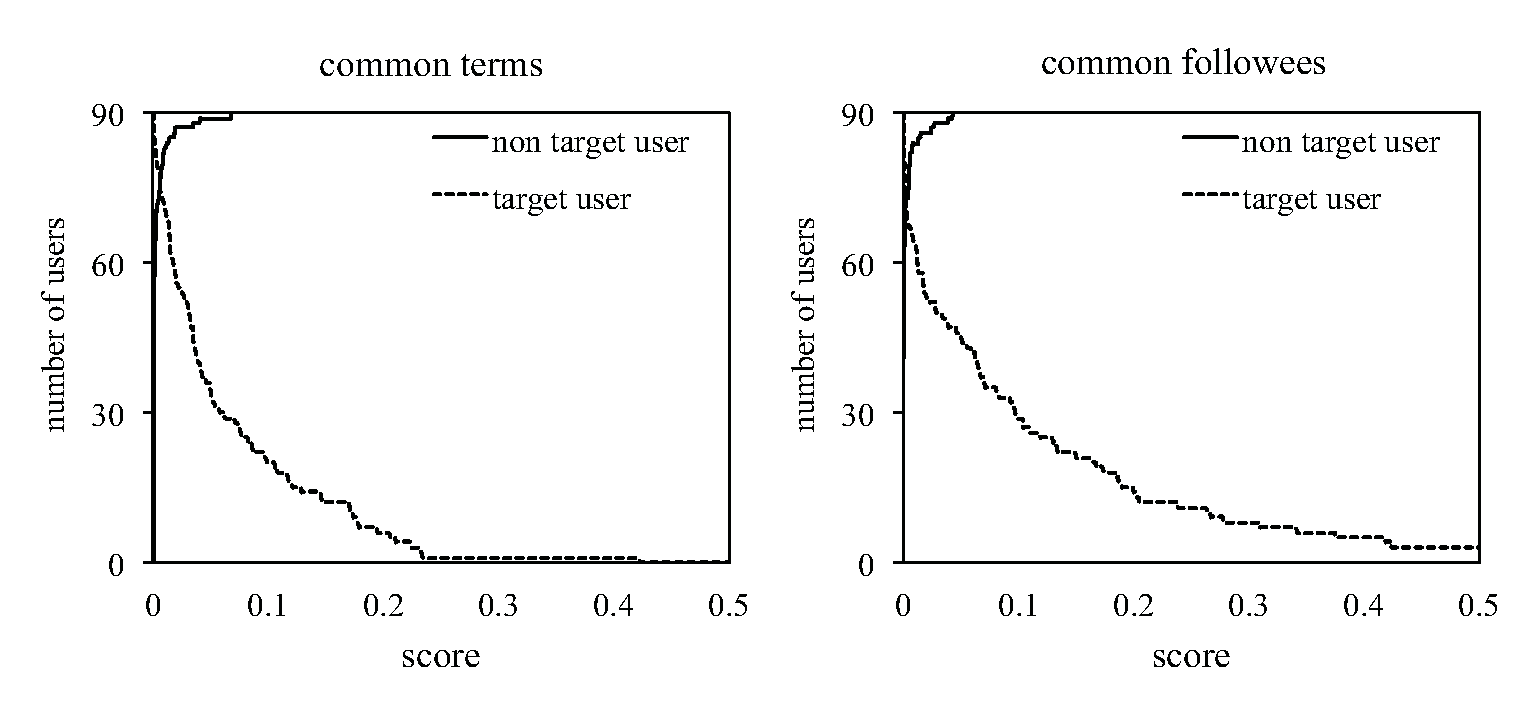
\includegraphics[width=14cm]{images/cumulativehistogram.eps}
 \caption{The cumulative histogram of specificity scores of each
 attribute on target users and non target users}
\label{fig:cumulativehistogram}
\end{center}
\end{figure}
}

{\footnotesize
\begin{figure}[t]
\begin{center}
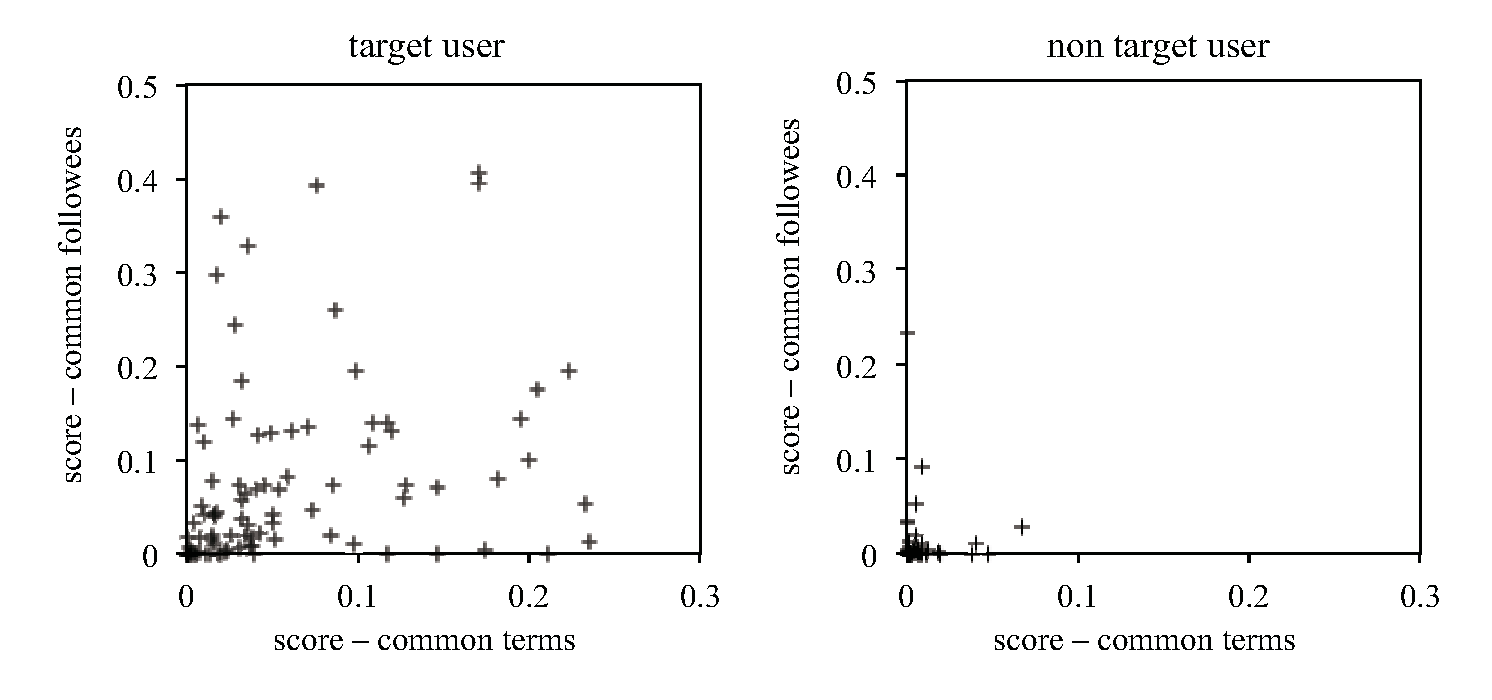
\includegraphics[width=14cm]{images/distribution.eps}
 \caption{A scatter diagram based on specificity scores of a couple of
 attributes, common terms and common followees, on target users and non
 target users}
\label{fig:distribution}
\end{center}
\end{figure}
}

\begin{table}[t]
\caption{Precision of the final classification of target users and non
 target users \label{table:Final Precision}}
\begin{center}
\begin{tabular}{cIcc|cccc}
 & \multicolumn{2}{c|}{Baseline} & \multicolumn{4}{c}{Proposed Method} \\
 \makebox[5em]{Method} & \makebox[4em]{follower} & \makebox[3em]{SVM} &
 \makebox[3em]{max} & \makebox[3em]{avg} & \makebox[4em]{SVM} &
 \makebox[4em]{decision tree} \\ \bhline{1.5pt}
 Precision & 0.878 & 0.828 & 0.856 & 0.872 & {\bf 0.944} & 0.906 \\
\end{tabular}
\end{center}
\end{table}

\begin{table}[t]
\caption{Details of the results of a part of users
 \label{table:Details}}
\begin{center}
\scalebox{0.75}{
\begin{tabular}{ccccccc}
 user  & term \& followee & $\mathit{local rate}$ &
 $\mathit{global rate}$ & $\mathit{SubsetScore}$ &
 $\mathit{SpecificityScore}$ \\ \bhline{1.5pt}
 target user & & & & & \\ \hline
 @MCstaff\_Fukuoka & Fukuoka & 0.563 & 0.047 & 0.390 & \\
 & music & 0.114 & 0.096 & 0.076 & 0.235 \\
 & Hakata & 0.095 & 0.003 & 0.076 & \\ \cline{2-7}
 & @fukuoka\_yokane & 0.069 & 0.023 & 0.046 &\\
 & @f\_sunpalace & 0.063 & 0.023 & 0.040 & 0.010 \\
 & @mbc\_o2\_eiji & 0.059 & 0.028 & 0.031 & \\ \hline
 @Jars0830 & Arashi & 0.439 & 0.039 & 0.304 & \\
 & participation & 0.190 & 0.026 & 0.131 & 0.233 \\
 & line & 0.130 & 0.045 & 0.090 & \\ \cline{2-7}
 & @Yamnos5 & 0.249 & 0.004 & 0.246  & \\
 & @ars\_762 & 0.109 & 0.072 & 0.037 & 0.067 \\
 & @nino\_xoxo\_ & 0.070 & 0.033 & 0.037 & \\ \hline
 @pa\_ko065 & piano & 0.528 & 0.009 & 0.366 & \\
 & music & 0.250 & 0.096 & 0.173 & 0.223 \\
 & Sapporo & 0.139 & 0.022 & 0.096 & \\ \cline{2-7}
 & @mofu\_co & 0.500 & 0.001 & 0.499  & \\
 & @miko3535 & 0.500 & 0.003 & 0.497 & 0.277 \\
 & @shimagaraneko & 0.472 & 0.002 & 0.470 & \\ \bhline{1.5pt}
 non target user & & & & & \\ \hline
 @masason & fan & 0.059 & 0.676 & 2.62e-17 \\
 & Tokyo & 0.027 & 0.196 & 0 & 1.20e-12 \\
 & music & 0.024 & 0.096 & 1.34e-15 & \\ \cline{2-7}
 & @shigeruishiba & 0.050 & 0.939 & 0 & \\
 & @WSJJapan & 0.066 & 3.56 & 0 & 0 \\
 & @HeizoTakenaka & 0.05 & 3.62 & 0 & \\ \hline
 @Kantei\_Saigai & Tokyo & 0.034 & 0.196 & 0 & \\
 & hobby & 0.027 & 0.095 & 1.14e-15 & 3.52e-9 \\
 & movie & 0.019 & 0.043 & 1.85e-7 & \\ \cline{2-7}
 & @MofaJapan\_ITPR & 0.056 & 0.597 & 0 & \\
 & @CAO\_BOUSAI & 0.203 & 0.834 & 0 & 0.001 \\
 & @MofaJapan\_jp & 0.062 & 0.950 & 0 & \\ \hline
 @tenkijp & Tokyo & 0.033 & 0.196 & 0 & \\
 & hobby & 0.022 & 0.095 & 9.28e-16 & 2.51e-5 \\
 & music & 0.021 & 0.096 & 1.18e-15 & \\ \cline{2-7}
 & @tenkijp\_jishin & 0.421 & 10.4 & 0  & \\
 & @Kantei\_Saigai & 0.358 & 14.8 & 0 & 0 \\
 & @bouei\_saigai & 0.277 & 6.31 & 0 & \\ \hline
\end{tabular}
}
\end{center}
\end{table}

\subsection{Results and Evaluation of Classifying Users of High Target
  Specificity}
\label{subsec:Results of Method2}

In this subchapter, we show the results of the experiments classifiying
target users.  Table~\ref{table:Precision} shows the precision of four
types of classification methods: a combination of two approaches and two
classifiers, i.e., a 3-class SVM, 2 binary SVMs, a 3-class decision
tree, and 2 binary decision trees, with all features mentioned in
\ref{sec:ClassificationMethod2} into three categories.  The precision
of classification methods using SVMs as classifiers are more than 10
points higher than that using decision trees.  When using SVMs as
classifiers, the precision of 2 binary classifiers are a little higher
than that of a 3-class classifier, and it is the opposite when using
decision trees.  But for both methods using SVMs and decision trees, the
difference between the precision of 2 binary classifiers and that of a
3-class classifier is not so big, which suggests that the two causes of
the high target specificity mentioned in \ref{subsec:The Causes} are
highly independent of each other.

Next, we show the details of the results of classification methods using
SVMs as classifiers.  The second column of Table~\ref{table:Classifier
Details} shows the precision of each classification method with all
features, and the following columns show the precision when we remove
each feature from the data.  Each feature of i, ii, iii, and iv
correspond to those in \ref{sec:ClassificationMethod2} respectively.
For each method, a bold number shows when the precision becomes the
lowest.

The socond and third rows show the precision of a 3-class SVM
and 2 binary SVMs respectively.  For each method, the precision became
the lowest when we removed the feature (i): numbers of followees and
followers, and their ratio.  It is able to be said that numbers of
followees and followers, and their ratio are mainly useful for
determining the cause of high target specificity.  The precision also
became lower to some extent when we removed the feature (iv):
partialness of topics in messages.  This suggests that partialness of
topics in messages is related to high target specificity.
Table~\ref{table:topics} shows a part of topics out of 20 extracted by
LDA.  We were able to extract topics about news programs, disasters, and
so on.  On the other hand, the precision became higher when we removed
the feature (ii): mutual follow ratio.  This suggests that mutual
follow ratio and whether the user publishes information to the closed
users are not necessarily correlating.

The fourth and fifth rows show the precision of each binary SVM used for
the method of 2 binary SVMs: a SVM determining whether users publish
information specified for certain topics, and that determining users
publish information to the users specified extensionally, respectively.
The precision of the former became the lowest when we removed the
feature (i): numbers of followees and followers, and their ratio, and
that of the latter became the lowest when we removed the feature
(iv): partialness of topics in messages, which is the noticeable
metter.  This suggests that partialness of topics is more useful for
determing whether users publish information to the users specified
extensionally or not than whether users publish information specified
for certain topics or not.

\begin{table}[t]
\caption{Precision of the classification of target users
 \label{table:Precision}}
 \begin{center}
\begin{tabular}{cIc|c}
 & \makebox[6em]{SVM} & \makebox[6em]{decision tree} \\ \bhline{1.5pt}
 \makebox[10em]{3-class classifier} & 67.8 & 55.6 \\ \hline
 2 binary classifiers & {\bf 68.9} & 53.3 \\
\end{tabular}
 \end{center}
\end{table}

\hdashlinewidth=0.5mm
\begin{table}[t]
\caption{Precision of SVMs without each feature \label{table:Classifier
 Details}}
\begin{center}
\begin{tabular}{ccIc|cccc}
 \multicolumn{2}{cI}{Removed Feature} & \makebox[4em]{with all} &
 \makebox[3em]{i} & \makebox[3em]{ii} & \makebox[3em]{iii} &
 \makebox[3em]{iv} \\ \bhline{1.5pt}
 \multicolumn{2}{cI}{3-class SVM} & 67.8 & {\bf 64.4} & 72.2 & 67.8 &
 65.5 \\ \hline
 \multicolumn{2}{cI}{2 binary SVMs} & 68.9 & {\bf 65.6} & 71.1 & 67.8 &
 67.8 \\ \hdashline
 \makebox[4em]{} & \makebox[3em]{topic} & 85.6 & {\bf 81.1} & 86.7 & 84.4 & 84.4 \\
 \makebox[4em]{} & \makebox[3em]{user} & 83.3 & 84.4 & 84.4 & 83.3 & {\bf 82.2} \\
\end{tabular}
\end{center}
\end{table}

\begin{table}[t]
\caption{A part of topics extracted by LDA
 \label{table:topics}}
\begin{center}
\begin{tabular}{c|c}
topic id & \makebox[25em]{words} \\ \bhline{1.5pt}
1 & news, program, broadcast, morning, night, tonight \\
2 & update, blog, picture, smart phone, weather\\
3 & worst, typhoon, Sea of Japan, electricity \\
4 & earthquake, observation, focus, concern, teacher \\
\end{tabular}
\end{center}
\end{table}